%*******10********20********30********40********50********60********70********80
\chap{Background Theory}
    
\section{Agile Software Development} \label{Agile}
\vspace{-5mm}
Agile is an umbrella term for methods of software development, based on the idea of developing software incrementally, instead of all at once. The project itself is broken down into several \textit{user stories}, where each story gets a weighted value based on difficulty. The stories are divided into short cycles called \textit{iterations}.\cite{agile:nutshell}

\subsection{User stories}
\vspace{-5mm}
User stories are very high-level definitions of project requirements, and contain just enough information so the developers can estimate a time frame for completing it. The usual format of a user story looks somewhat like this:
\vspace{-5mm}
\begin{center}
	\textit{As a (role) I want (something) so that (benefit).}
\end{center}
\vspace{-5mm}
Each story is expected to yield a contribution to the overall completion if the product.\cite{agile:modeling}

\pagebreak
\subsection{Iterations}\label{iter}\vspace{-5mm}
An iteration is a short period of time where some of the user stories are implemented completely. This means that for each iteration a new part of the project is fully implemented and tested. Each iteration usually consists of different renditions of these parts: plan, design, build, test, and review. 
\begin{figure}[H]
	\centering
	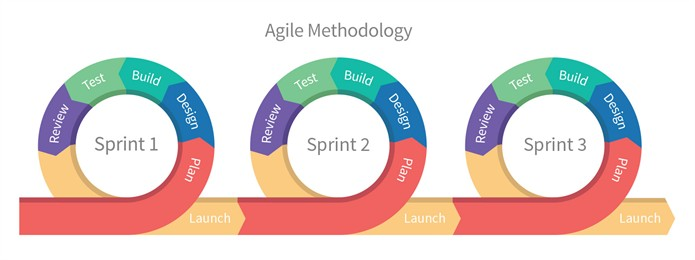
\includegraphics[trim={0 0 0 0},clip,width=0.8\textwidth]{Files/agile.jpg}
	\caption{Visualization of the iterations\cite{agile:figure}.}
	\label{fig: MVC}
\end{figure}

\section{Ruby on Rails} 
\vspace{-5mm}
Ruby on Rails (RoR) is a server-side web application framework. RoR is a model–view–controller framework, providing default structures for a database, a web service, and web pages.\cite{wiki:RoR}

\begin{figure}[H]
	\centering
    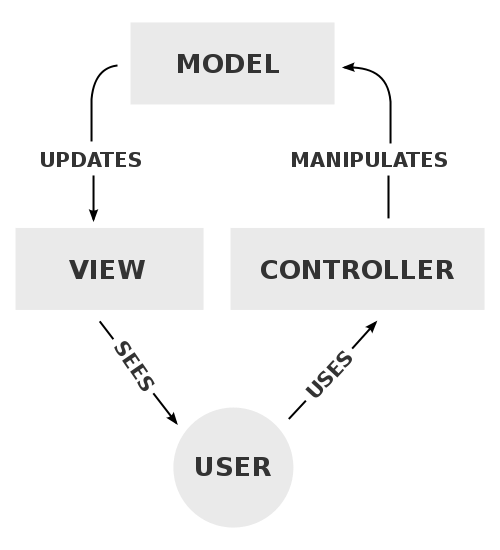
\includegraphics[trim={0 0 0 0},clip,width=0.4\textwidth]{Files/MVC.png}
    \caption{Diagram of interactions within the MVC pattern.\cite{wiki:mvc} }
    \label{fig: MVC}
\end{figure}
\vspace{-3mm}

\textbf{The Model} contains the data and the state if the application, and it has no knowledge of the user interface, so it can be reused.\\
\textbf{The View} generates the user interface which presents the user with the data, but isn't able to do any processing. Different views are able to access the same model for different usages.\\
\textbf{The Controller} interacts with the outside world through the views, interacts with the model, and displays the appropriate view to the user.




